% ========== MINK ==========
\begin{frame}{%
  \begin{minipage}[c]{0.30\textwidth}
    Mink
  \end{minipage}%
  \hfill
  \begin{minipage}[c]{0.45\textwidth}
    \footnotesize
    \textbf{Jagttid:} 1. sep -- 31. jan\\
    \textbf{Regulering:} Uden aftale (invasiv)
  \end{minipage}%
  \hfill
  \begin{minipage}[c]{0.15\textwidth}
    \noindent\raggedleft
    
\includegraphics[width=0.5cm, height=0.5cm, keepaspectratio]{Billeder/Ikoner/star.png}%
    \hspace{0.2em}%
    
\includegraphics[width=0.5cm, height=0.5cm, keepaspectratio]{Billeder/Ikoner/star.png}
  \end{minipage}%
}
  \vspace{0.25em}
  \begin{columns}[T]
    % --- Venstre kolonne: Tekst ---
    \column{0.45\textwidth}
    \setlength{\parskip}{0.4em}
    \tiny
    \RaggedRight
    \textbf{\textit{Neogale vison}} – undslupne dyr fra pelsavl har etableret sig langs kysterne mange steder i Danmark. \par
    \textbf{Udseende:}\\
    \quad – Mørk, ensfarvet pels \\
    \quad – Vilde mink kan være lysere ved hovedet \\
    \quad – Ingen maske som ilderen \par
    \textbf{Levesteder:} I nærheden af vand. \par
    \textbf{Føde:} Fisk, smågnavere, fugle, krabber, padder og insekter. \par
    \textbf{Udbredelse:} Hele landet undtagen småøer.
    % --- Højre kolonne: Større billede ---
    \column{0.52\textwidth}
    \centering
    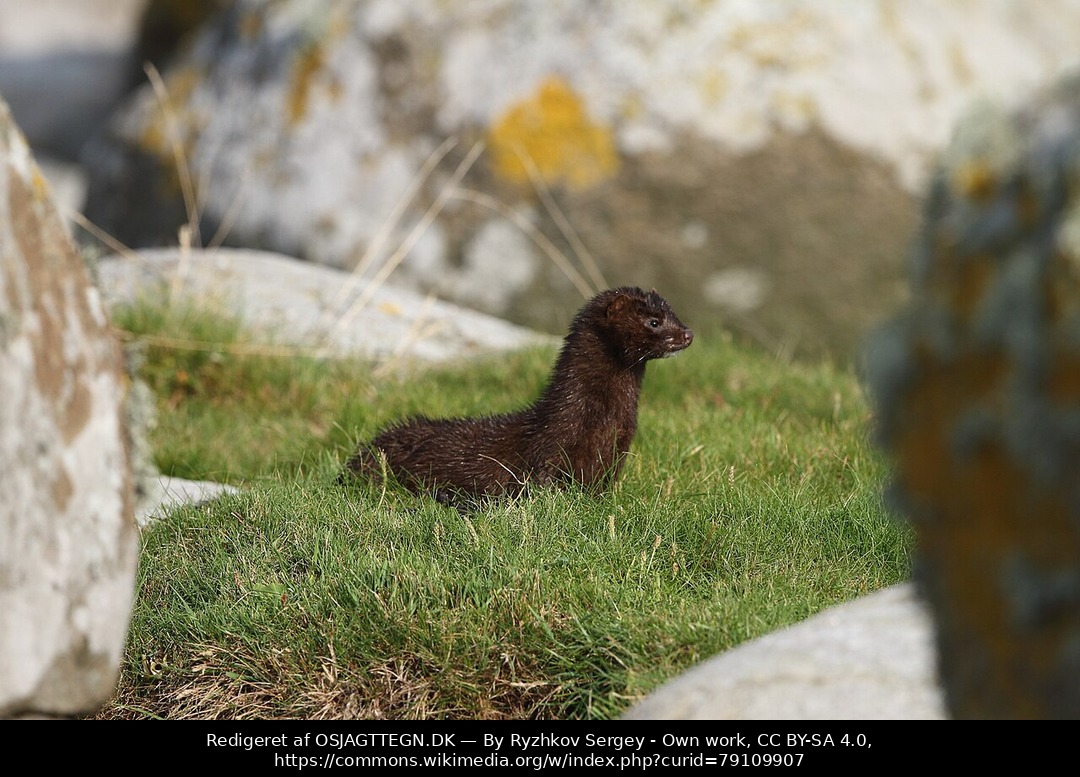
\includegraphics[width=\linewidth, height=7.2cm, keepaspectratio]{Billeder/Dyr/Pattedyr/rovdyr/mink/mink-01.jpg}
  \end{columns}
\end{frame}